\documentclass[a4paper,12pt]{article}
\usepackage[hidelinks]{hyperref}
\usepackage{graphicx}
\usepackage{float}
\usepackage{caption}
\usepackage{array}
\usepackage{tabu}

%% Title Page 
\begin{document}
\title{\Huge Functional Requirements Document Specification \\ 
	 Project: \\ 
	Cafeteria Management System: Resolve}
\author{
         \underline{T-RISE}\\
          Rendani Dau (13381467) \\
	Elana Kuun (12029522) \\
	Semaka Malapane (13081129) \\
	Antonia Michael (13014171) \\
	Isabel Nel (13070305)\\ \\
	https://github.com/toniamichael94/MainProjectCOS301}

\date{\today}
 
%\documentclass[12pt]{article}


\maketitle
\break

%% Make table of contents
\tableofcontents
\break

\begin{tabu} to 0.8\textwidth { | X[l] | X[l] | }
 \hline
\textbf{Document Title} & Functional Requirements Document \\
 \hline
 \textbf{Document Identification}  & Document 0.0.4 \\
\hline
 \textbf{Author}  & Rendani Dau, Elana Kuun, Semaka Malapane, Antonia Michael, Isabel Nel \\
\hline
\textbf{Version} & 0.0.4 \\
\hline
\textbf{Document Status} & Fourth Version - edited the whole document thoroughly, added Manage System module and made other module changes and additions \\
\hline
\end{tabu}

\begin{table}[h!]
\centering
 \begin{tabular}{||c c c c||} 
 \hline
 \textbf{Version} & \textbf{Date} & \textbf{Summary} & \textbf{Authors} \\ [0.5ex] 
 \hline\hline
 0.0.1 & 29 May 2015 &  First draft contains first two use cases  & Rendani Dau, \\ & & & Elana Kuun, \\ & & & Semaka Malapane, \\ & & & Antonia Michael \\ & & & Isabel Nel, \\ & & & \\
 \hline 
 & & & \\
 0.0.2 & 6 July 2015 &  Second draft adding Register & Rendani Dau, \\ & & and Authentication use & Elana Kuun, \\ & & cases and updated profile & Semaka Malapane, \\ & & &  Antonia Michael \\ & & & Isabel Nel \\   [1ex] 
 \hline
& & & \\
 0.0.3 & 22 July 2015 &  Third draft adding Inventory & Rendani Dau, \\ & & and Menu use & Elana Kuun, \\ & & cases  & Semaka Malapane, \\ & & &  Antonia Michael \\ & & & Isabel Nel \\   [1ex] 
 \hline
& & & \\
 0.0.4 & 23 July 2015 &  Fourth draft adding Manage & Rendani Dau, \\ & & system and editing & Elana Kuun, \\ & & whole document  & Semaka Malapane, \\ & & &  Antonia Michael \\ & & & Isabel Nel \\   [1ex] 
\hline
 \end{tabular}
\end{table}

\pagebreak



%%now begin document

%%---------------------------------  INTRODUCTION -------------------------------------------
\section{Introduction}
This document contains the functional requirements specification, architecture requirements and testing for the Resolve Cafeteria Management System that will be created for Software Engineering (COS 301) at the University of Pretoria 2015, by the group T-RISE. In this document we will thoroughly discuss and layout the project's functional requirements to provide a clear view of the system as a whole. An agile approach is being followed which involves an interactive and incremential method of managing and designing the system. 
%% ------------------------------ VISION ------------------------------------------------------
\section{Vision}
The vision of this project is to implement a flexible, pluggable, fully functional software application that will be maintainable, with detailed supporting documentation and an instruction manual for the Cafeteria Management System. This system will assist in managing the cafeteria's inventory/stock, placing orders made by employees, generating bills, and sending the appropriate information to the right parties.  

%%---------------------------------- BACKGROUND -----------------------------------------
\section{Background}
As specified in the project proposal document from Resolve, the cafeteria is currently cash only and does not accept bank cards or electronic payments. This makes it inconvenient for employees as they have to have cash on hand if they want to purchase anything from the cafeteria. Employees might choose to buy somewhere else where they can use another form of payment. The employees have to use fuel and time, and this does not bring in the maximum amount of income to the cafeteria, hindering its growth and improvement.\\

Resolve is therefore looking for a means to accept payments from employees for the canteen using their employee access cards or access card numbers. The amount spent at the cafeteria can then be deducted from their salary at the end of the month.\\

After our first meeting with the client, they brought to our attention that at times the cafeteria does not have enough stock to provide some of the menu items, therefore the managing of inventory and stock will also be part of the system. The system will also predict what inventory/stock needs to be bought for the next week in order to avoid shortcomings. At the end of each month, the bill for that month will be sent to either payroll or to the employee. This option is configurable from the user's profile. The employee can also set a spending limit for each month. The system will also have a maximum limit that users cannot exceed.
 
%%--------------------------------------- FUNCTIONAL REQUIREMENTS--------------------------------
\section{Functional Requirements and Application Design}
In this section we will discuss the functional requirements. \\

%% ---------------USE CASES -------------------
\subsection{Use Cases }
Below is a list of all the use cases we have identified:

\begin{itemize}

\item Authentication
\item Manage System
\item Manage Profile
\item Place Order
\item Manage Cafeteria
\item Manage Inventory 

\end{itemize}


%% ---------------USE CASE PRIORITIZATION -------------------
\subsection{Use Case Prioritization}
Below the use cases mentioned above will be catagorized as critical, important or nice to have.

\begin{itemize}

\subsubsection{Critical}
\item Authentication \\
This is a critical use case due to the fact that you cannot send through any order if you are not logged in. In such a case you will only be able to view the menu. In addition, you can not log into the system if you have not been registered on the system.

\item Place Order\\
This is critical due to the fact that the main functionality of the system revolves around the ability to place orders at the cafeteria as well as other activities relating to that. 

\item Manage Inventory \\
This use case is considered critical because it deals with adding, removing, searching for and updating (i.e. incrementing stock that has been added and decrementing stock when it is purchased or expired). This is hence vital for achieving the purpose of the system. The items displayed on the menu will contain a field called "Not in stock" if there is not a sufficient supply of inventory for the various menu items. 

\item Manage Cafeteria \\
This use case is considered critical because it deals with firstly adding menu items to the menu that the user will view, which again is vital for achieving the purpose of the system, as well as removing, updating and searching for various menu items. 

\subsubsection{Important}
\item Manage Profile \\
This use case is considered important because the user must be able edit their profile by resetting their personal spending limits and changing their email and passwords. The user must also be able to view his/her account history and current bill. It is crucial that the user is able to configure spending limits according to their own preferences as well as keep track of monthly purchases.

\item Manage System \\
This use case is considered important because this is where the superuser will configure the maximum spending limit, assign roles such as a cashier, change employee IDs as well as branding functionality such as setting the canteen name and uploading a canteen photo for the home page.

\end{itemize}

%%--------------- USE CASE/SERVICE CONTRACTS --------------
\section{Modular System}
The system will be built using a modular approach to allow more modules to be added at a later stage. This will also provide for pluggability and integratibility of the system.

\subsection{High level use case diagram of the CMS}
\begin{figure}[H]
  \centering
    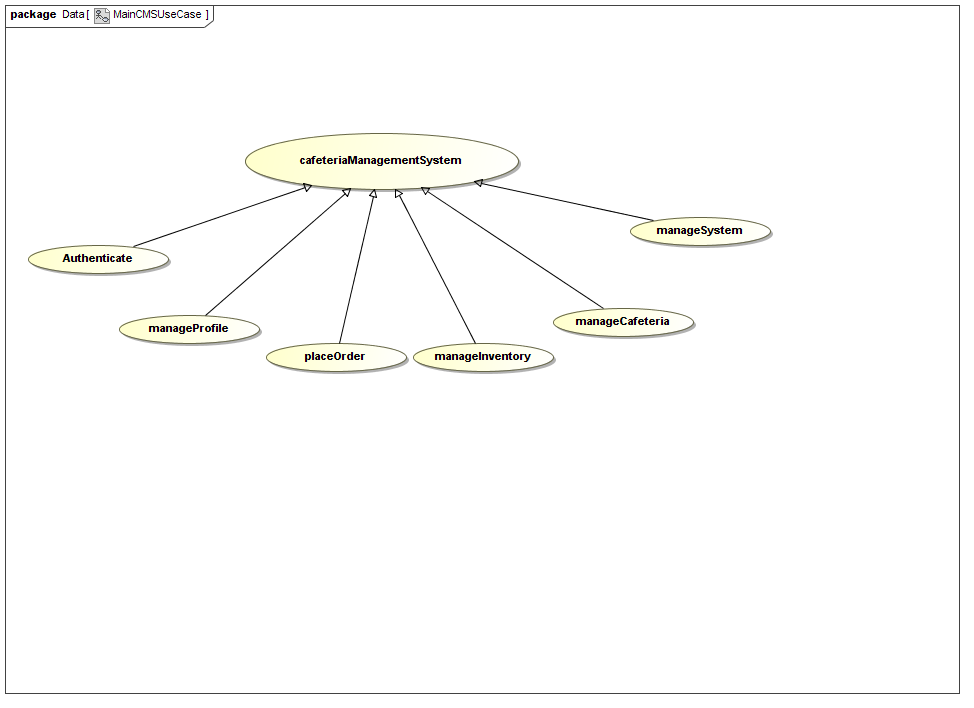
\includegraphics[width=1.0\textwidth]{../images/CMSUseCase.png}
    \caption{Cafeteria Management System Use Case} 
\end{figure}
The core of the system is a cafeteria management system that will provide functionality such as allowing users to place orders once they have registered and logged on to the system. Different types of users will have different privileges. 

\subsection{Authentication Module}
In this module, the functionality provided consists of validating the credentials entered into the system by a user whilst signing in. In addition, assistance is provided via the forgotPassword functionality. The different roles are also obtained in order to assign different functionality to users based on their roles. The register/ sign up functionality is also included here. 
\begin{figure}[H]
  \centering
    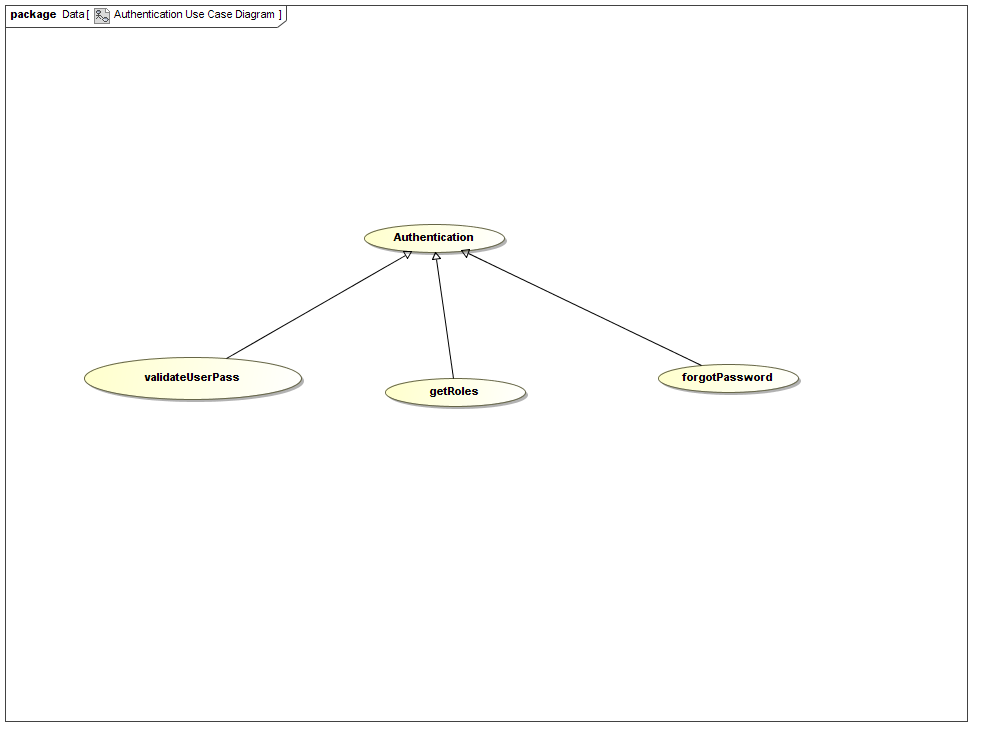
\includegraphics[width=1.0\textwidth]{../images/AuthenticationUseCaseDiagram.png}
    \caption{The main use case diagram for Authentication} 
\end{figure}

\subsubsection{Forgot Password }
The service contract and activity diagram for forgotPassword follow. forgotPassword falls under the use case for Authentication (refer to page 15 - figure 12 to view this use case diagram). Here, a user who has forgotten their password will be assisted via sending an email to the user's email account with steps to follow to create a new password.
\begin{figure}[H]
  \centering
    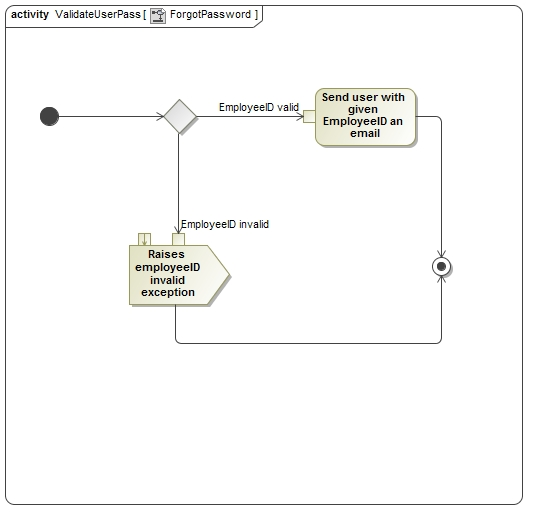
\includegraphics[width=1.0\textwidth]{../images/ForgotPassword.jpg}
    \caption{The activity diagram for forgotPassword} 
\end{figure}
\begin{figure}[H]
  \centering
    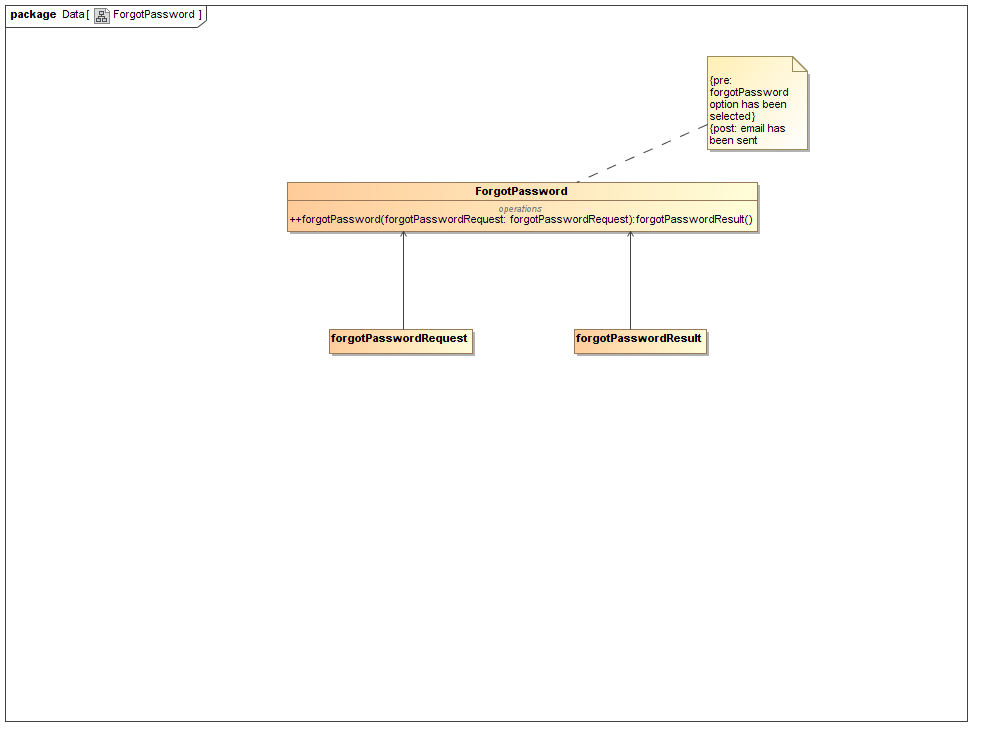
\includegraphics[width=1.0\textwidth]{../images/ForgotPassword.png}
    \caption{The service contract for forgotPassword} 
\end{figure}

\subsubsection{Validate User credentials }
The service contract and activity diagram for validateUserCredentials follow. validateUserCredentials falls under the use case for Authentication (refer to page 15 - figure 12 to view this use case diagram). Here, a user who has forgotten their password will be assisted via sending an email to the user's email account with steps to follow to create a new password.
\begin{figure}[H]
  \centering
    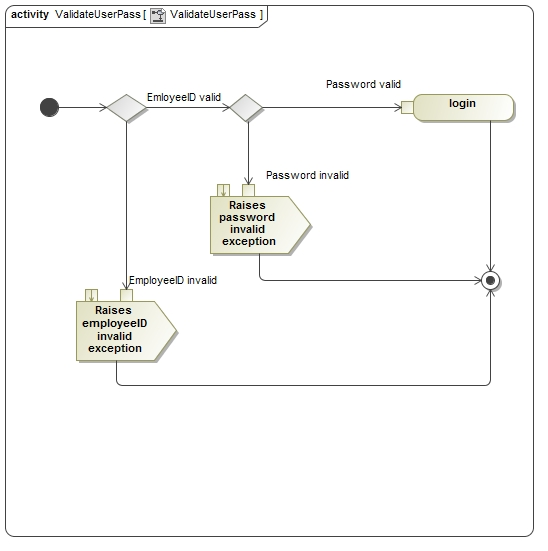
\includegraphics[width=1.0\textwidth]{../images/ValidateUserPass.jpg}
    \caption{The activity diagram for validateUserCredentials} 
\end{figure}
\begin{figure}[H]
  \centering
    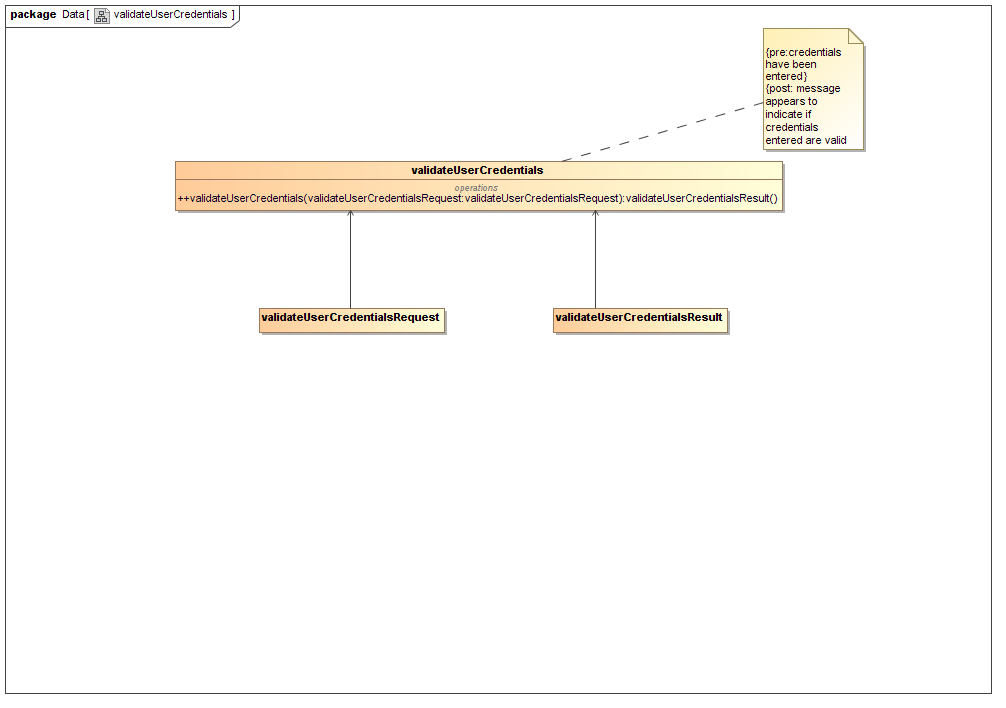
\includegraphics[width=1.0\textwidth]{../images/validateUserCredentials.png}
    \caption{The service contract for validateUserCredentials} 
\end{figure}

\subsubsection{Register }
Register provides the functionality to sign up as a user of the system. The user will set their limit, and personal details upon registration, as well as the recipient of their monthly bill. This is indicated in the following use case diagram.
\begin{figure}[H]
  \centering
    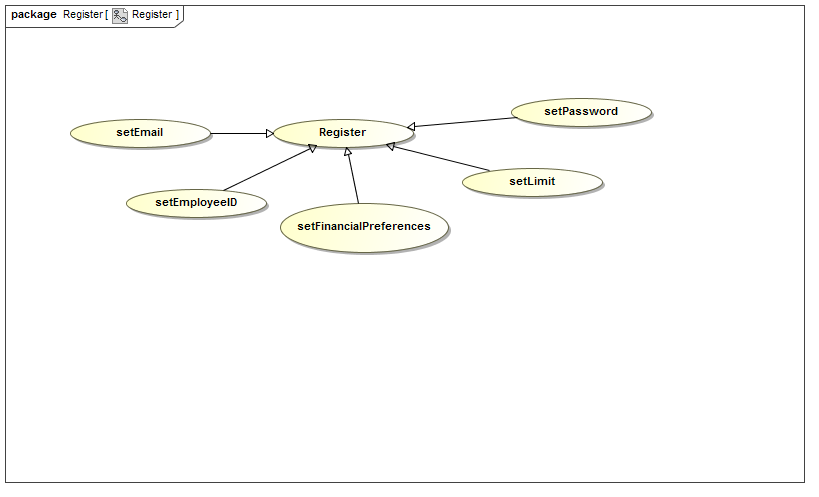
\includegraphics[width=1.0\textwidth]{../diagrams/Register/registerUseCase.png}
    \caption{The use case for registering on the system} 
\end{figure}
\subsubsection{Set email}
The service contract and activity diagram for setEmail follow. setEmail falls under the use case for Register (refer to page   - figure  to view this use case diagram). These details, entered by the user will be stored on the system.
\begin{figure}[H]
  \centering
    \includegraphics[width=1.0\textwidth]{../diagrams/Register/ActivityDiagrams/setEmail1.png}
    \caption{The activity diagram for setting an email address on the system} 
\end{figure}
\begin{figure}[H]
  \centering
    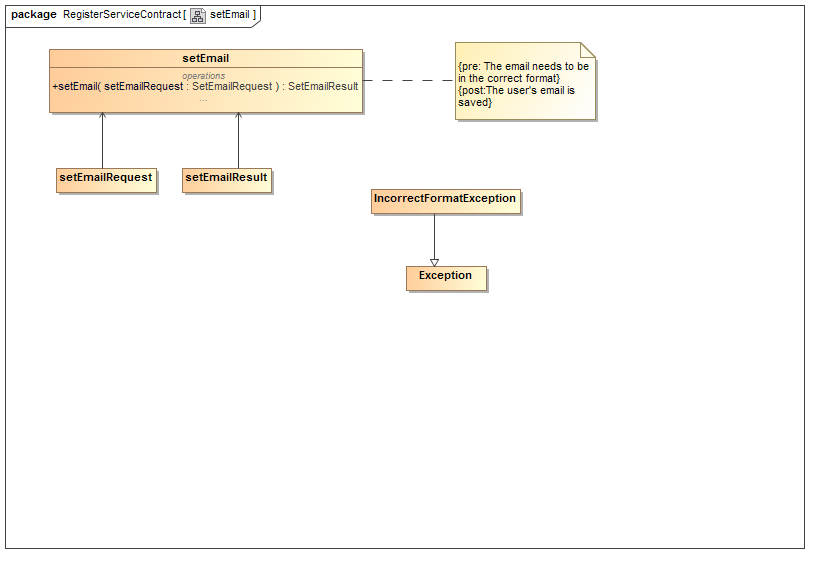
\includegraphics[width=1.0\textwidth]{../diagrams/Register/ServiceContractsRegister/setEmailServiceContract.png}
    \caption{The service contract for setting an email address on the system} 
\end{figure}

\subsubsection{Set Password}
The service contract and activity diagram for setPassword follow. setPassword falls under the use case for Register (refer to page 8 - figure 2 to view this use case diagram). These details, entered by the user will be stored on the system.
\begin{figure}[H]
  \centering
    \includegraphics[width=1.0\textwidth]{../diagrams/Register/ActivityDiagrams/setPassword1.png}
    \caption{The activity diagram for setting a password on the system} 
\end{figure}
\begin{figure}[H]
  \centering
    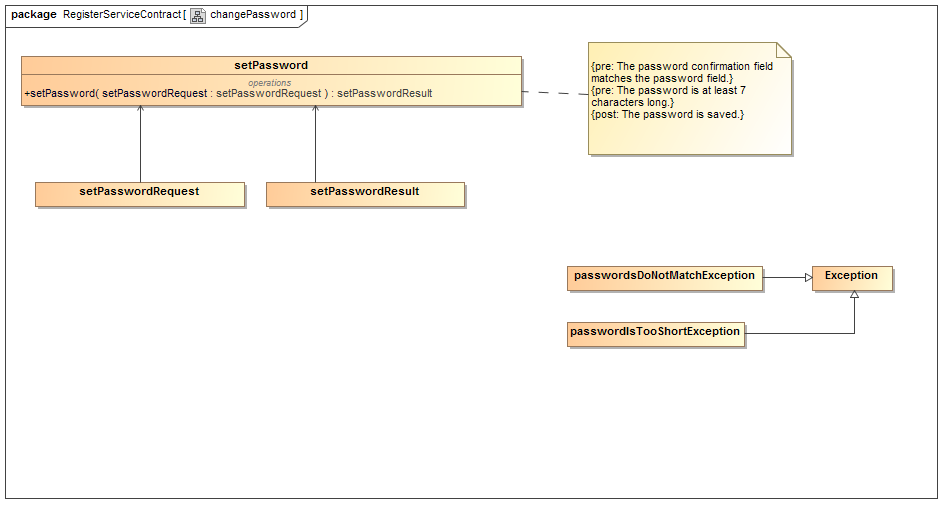
\includegraphics[width=1.0\textwidth]{../diagrams/Register/ServiceContractsRegister/changePasswordServiceContract.png}
    \caption{The service contract for setting a password on the system} 
\end{figure}

\subsubsection{Set Limit}
The service contract and activity diagram for setLimit follow. setLimit falls under the use case for Register (refer to page 8 - figure 2 to view this use case diagram). These details, entered by the user will be stored on the system. 
\begin{figure}[H]
  \centering
    \includegraphics[width=1.0\textwidth]{../diagrams/Register/ActivityDiagrams/setLimit.png}
    \caption{The activity diagram for setting a limit on the system} 
\end{figure}
\begin{figure}[H]
  \centering
    \includegraphics[width=1.0\textwidth]{../diagrams/Register/ServiceContractsRegister/setLimit.png}
    \caption{The service contract for setting a limit on the system} 
\end{figure}

\subsubsection{Set Employee ID }
The service contract and activity diagram for setEmployeeID follow. setEmployeeID falls under the use case for Register (refer to page 8 - figure 2 to view this use case diagram). These details, entered by the user will be stored on the system.
\begin{figure}[H]
  \centering
    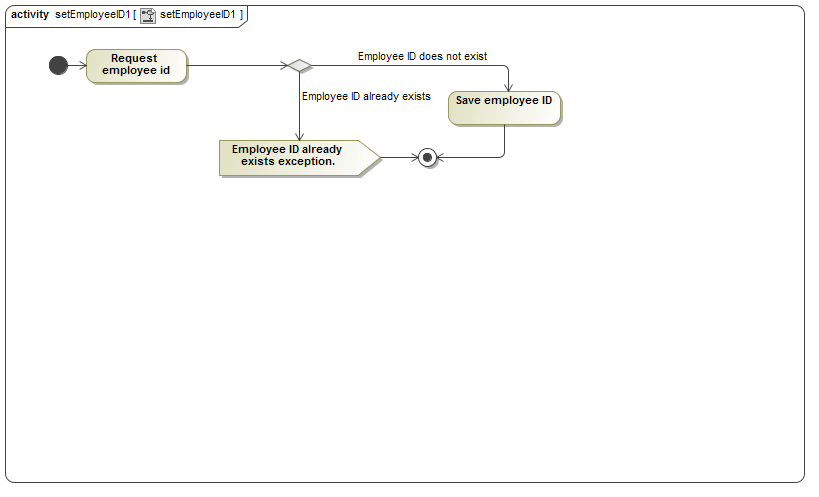
\includegraphics[width=1.0\textwidth]{../diagrams/Register/ActivityDiagrams/setEmployeeID1.png}
    \caption{The activity diagram for setting an employeeId on the system} 
\end{figure}
\begin{figure}[H]
  \centering
    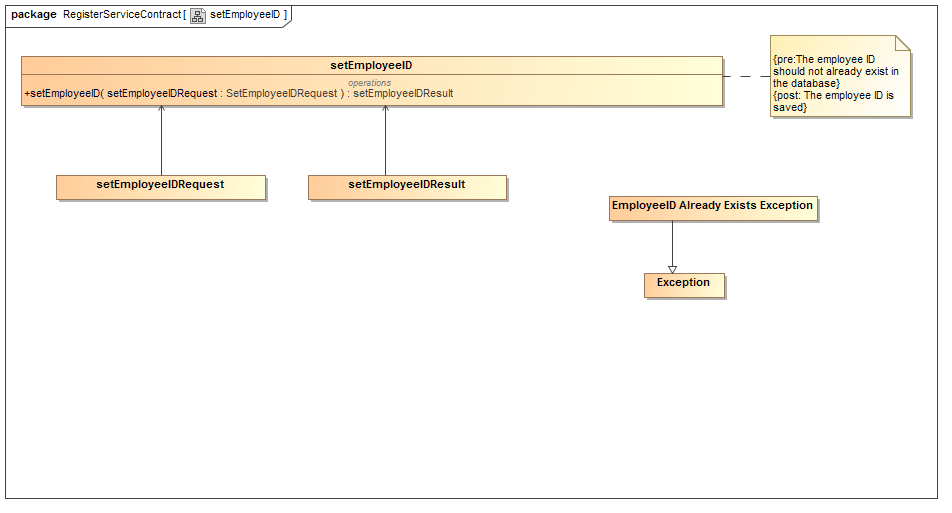
\includegraphics[width=1.0\textwidth]{../diagrams/Register/ServiceContractsRegister/setEmployeeIDServiceContract.png}
    \caption{The service contract for setting an employeeId on the system} 
\end{figure}

\subsubsection{Set Financial Preferences }
The service contract and activity diagram for setFinancialPreferences follow. setFinancialPreferences falls under the use case for Register (refer to page 8 - figure 2 to view this use case diagram). These details, entered by the user will be stored on the system.
\begin{figure}[H]
  \centering
    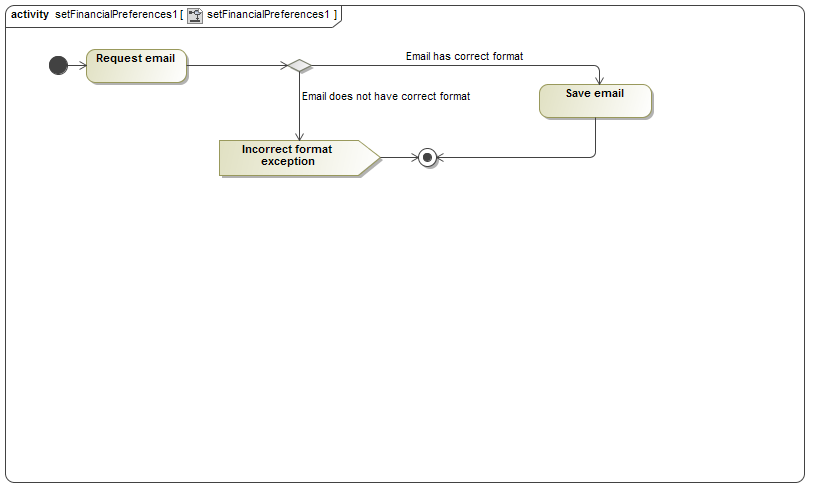
\includegraphics[width=1.0\textwidth]{../diagrams/Register/ActivityDiagrams/setFinancialPreferences1.png}
    \caption{The activity diagram for setting financial preferences on the system} 
\end{figure}
\begin{figure}[H]
  \centering
    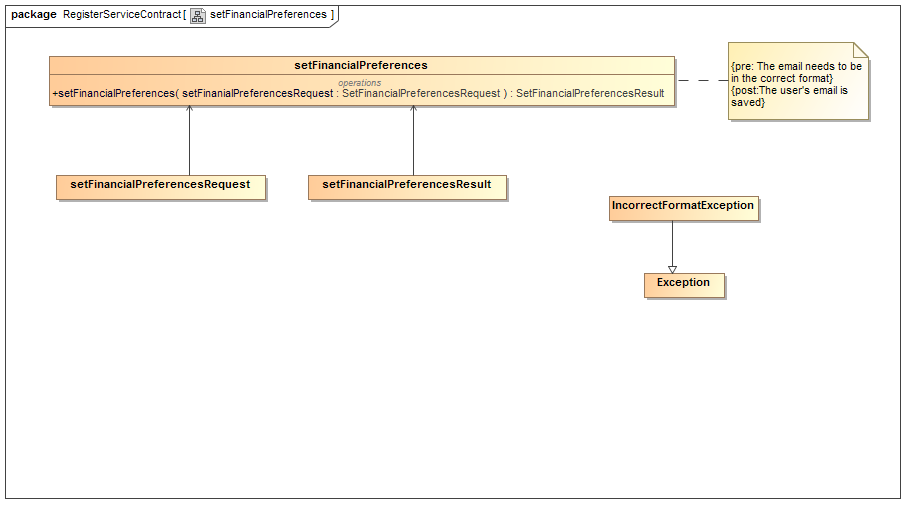
\includegraphics[width=1.0\textwidth]{../diagrams/Register/ServiceContractsRegister/setFinancialPreferencesServiceContract.png}
    \caption{The service contract for setting financial preferences on the system} 
\end{figure}

\subsection{Manage Cafeteria Module}
The menu module consists of the functionality of adding and removing meal items from the menu from which the user will place orders. This use case diagram indicates the functionality that this module consists of such as addMenuItem, updateMenuItem, searchMenuItem and deleteMenuItem, which are the use cases of this module.
\begin{figure}[H]
  \centering
    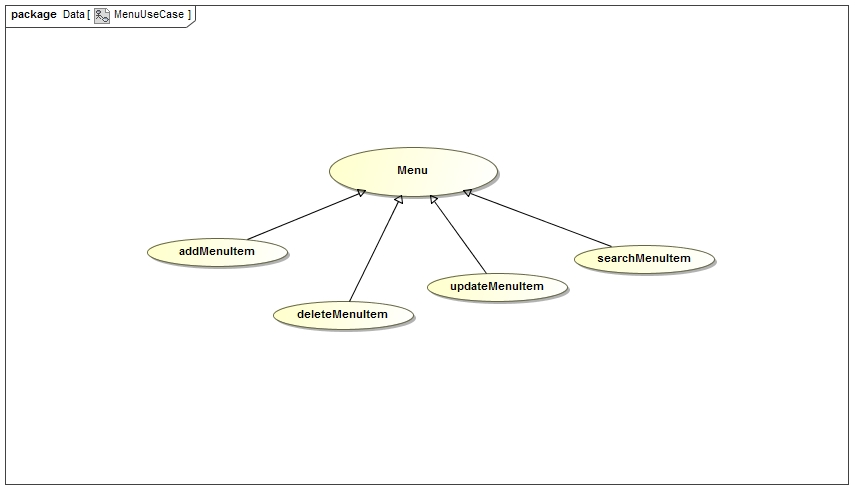
\includegraphics[width=1.0\textwidth]{../images/MenuUseCase.jpg}
    \caption{The use case for menu} 
\end{figure}
 \subsubsection{addMenuItem}
The service contract and activity diagram for addMenuItem follow. addMenuItem falls under the use case for Menu (refer to page   - figure   to view this use case diagram). The system allows the cafeteria manager to add items to the menu via the menu managing page.
\begin{figure}[H]
  \centering
    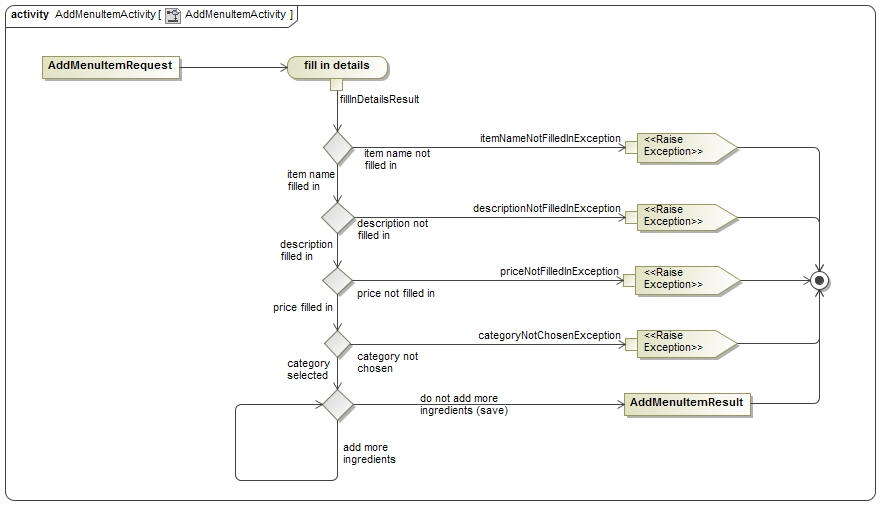
\includegraphics[width=1.0\textwidth]{../images/AddMenuItemActivity.jpg}
    \caption{The activity diagram for adding a menu item } 
\end{figure}
\begin{figure}[H]
	\centering
	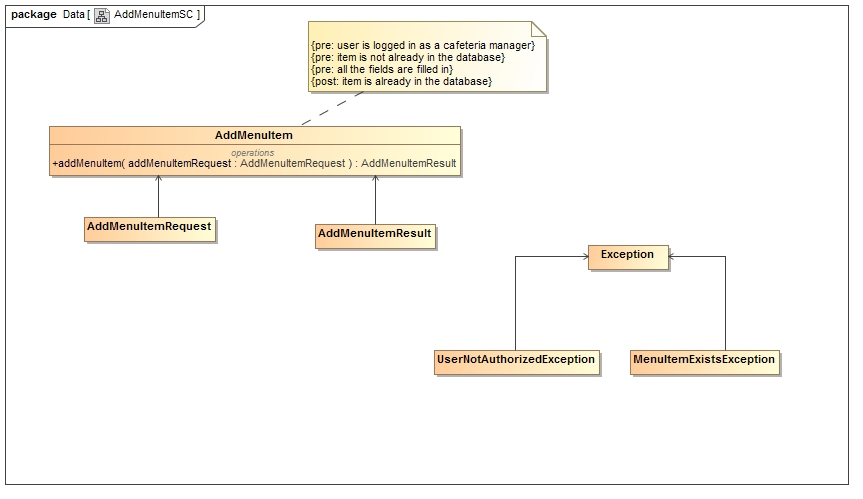
\includegraphics[width=1.0\textwidth]{../images/AddMenuItemSC.jpg}
	\caption{The service contract for adding a menu item}
\end{figure}

 \subsubsection{deleteMenuItem}
The service contract and activity diagram for deleteMenuItem follow. deleteMenuItem falls under the use case for Menu (refer to page   - figure   to view this use case diagram). The system allows the cafeteria manager to delete items from the menu via the menu managing page.
\begin{figure}[H]
  \centering
    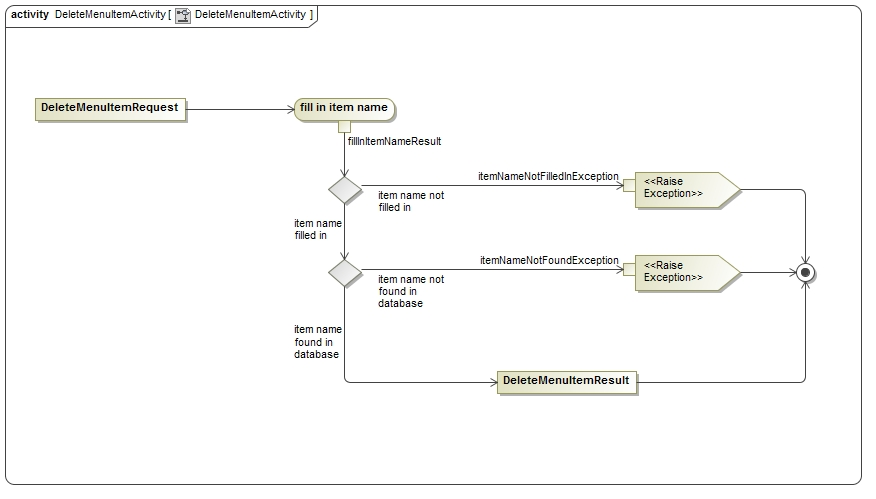
\includegraphics[width=1.0\textwidth]{../images/DeleteMenuItemActivity.jpg}
    \caption{The activity diagram for deleting a menu item } 
\end{figure}
\begin{figure}[H]
	\centering
	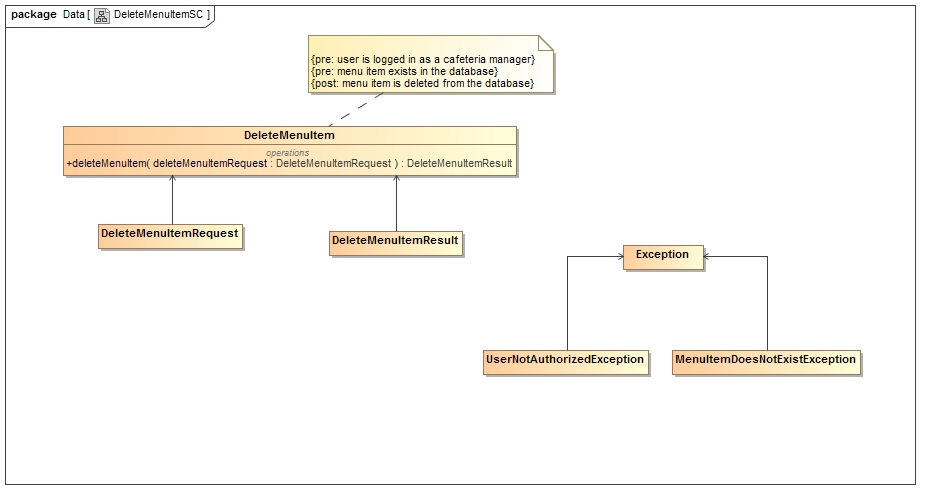
\includegraphics[width=1.0\textwidth]{../images/DeleteMenuItemSC.jpg}
	\caption{The service contract for deleting a menu item}
\end{figure}

 \subsubsection{searchMenuItem}
The service contract and activity diagram for searchMenuItem follow. searchMenuItem falls under the use case for Menu (refer to page   - figure   to view this use case diagram). The system allows the cafeteria manager to search for items from the menu via the menu managing page.
\begin{figure}[H]
  \centering
    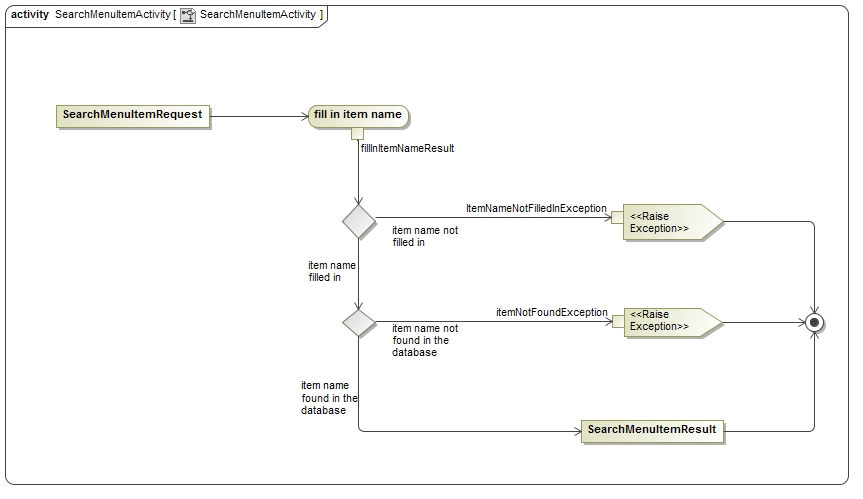
\includegraphics[width=1.0\textwidth]{../images/SearchMenuItemActivity.jpg}
    \caption{The activity diagram for searching for a menu item } 
\end{figure}
\begin{figure}[H]
	\centering
	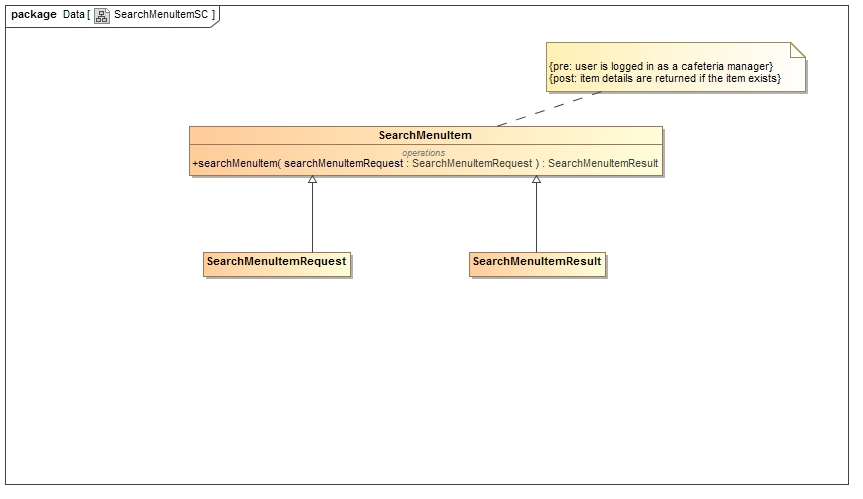
\includegraphics[width=1.0\textwidth]{../images/SearchMenuItemSC.jpg}
	\caption{The service contract for searching for a menu item}
\end{figure}

 \subsubsection{updateMenuItem}
The service contract and activity diagram for updateMenuItem follow. updateMenuItem falls under the use case for Menu (refer to page   - figure   to view this use case diagram). The system allows the cafeteria manager to update menu items' unit, quantity and name via the menu managing page.
\begin{figure}[H]
  \centering
    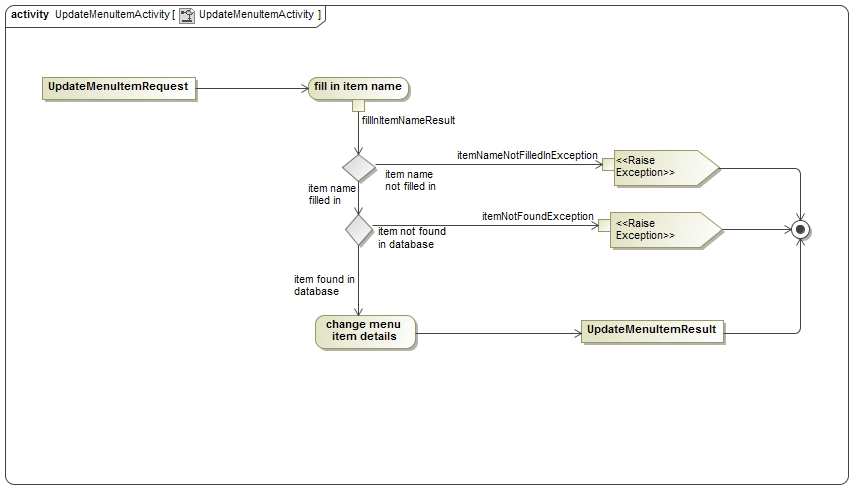
\includegraphics[width=1.0\textwidth]{../images/UpdateMenuItemActivity.jpg}
    \caption{The activity diagram for updating a menu item } 
\end{figure}
\begin{figure}[H]
	\centering
	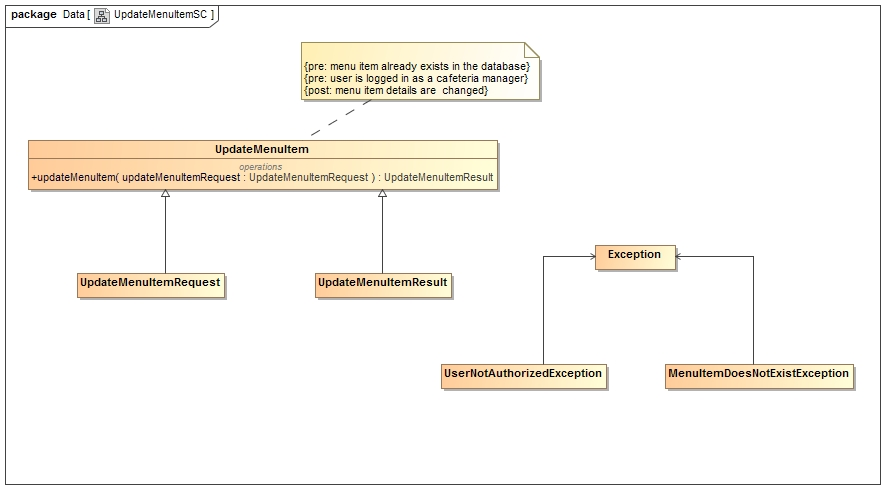
\includegraphics[width=1.0\textwidth]{../images/UpdateMenuItemSC.jpg}
	\caption{The service contract for updating a menu item}
\end{figure}

\subsection{Place Orders Module}
The main functionality the system serves to provide, is  to allow the user to use their access card number to purchase food items from the cafeteria via the system. This use case diagram indicates the functionality around placing orders, such as CheckProductAvailability and checkLimits, which are the use cases of this module.
\begin{figure}[H]
  \centering
    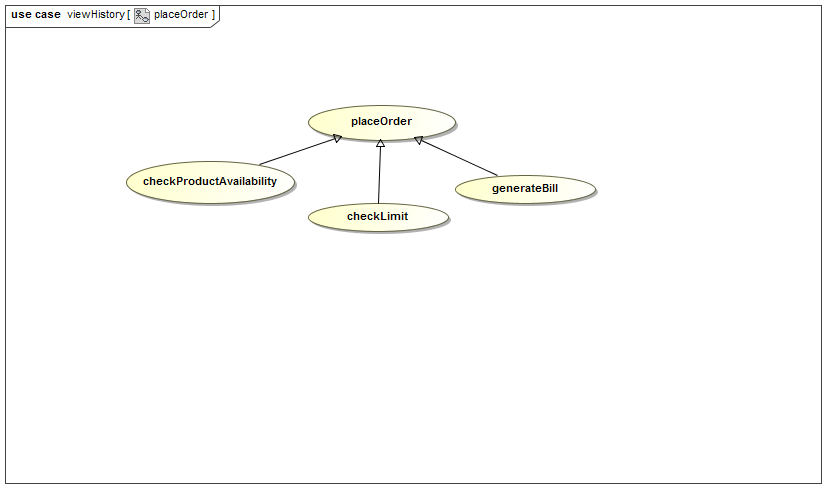
\includegraphics[width=1.0\textwidth]{../images/placeOrder.png}
    \caption{The use case for placing an order} 
\end{figure}
 
\subsubsection{CheckProductAvailability}
The service contract and activity diagram for CheckProductAvailability follow. CheckProductAvailability falls under the use case for Place Orders (refer to page 20 - figure 17 to view this use case diagram). The system will check whether the product that the user has selected to purchase is currently in stock.
\begin{figure}[H]
  \centering
    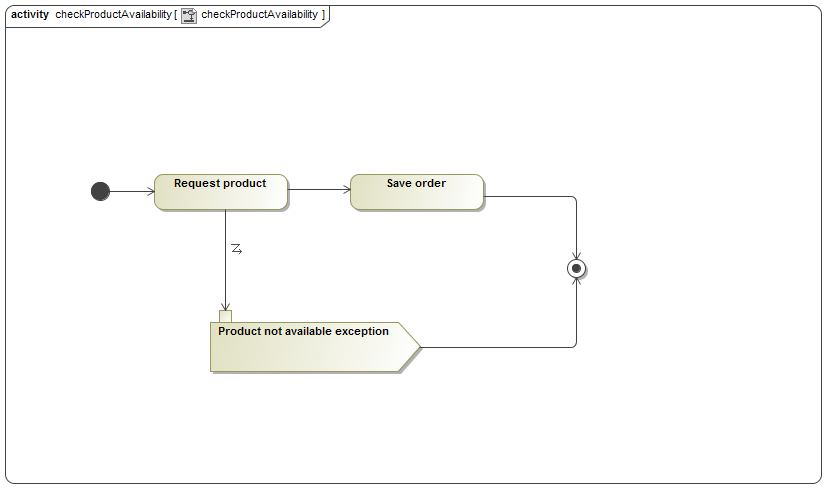
\includegraphics[width=1.0\textwidth]{../images/checkProductAvailability.png}
    \caption{The activity diagram for checking product availibilty } 
\end{figure}
 
\begin{figure}[H]
	\centering
	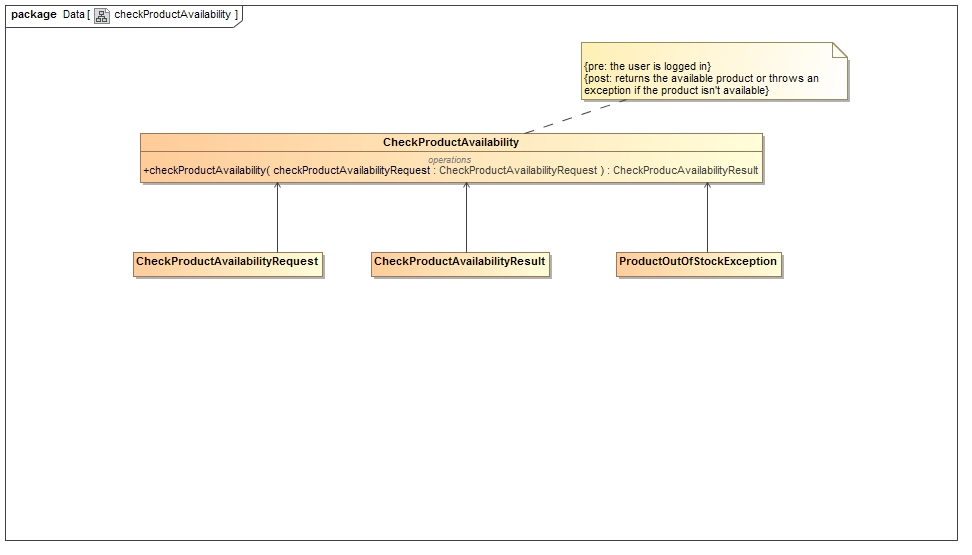
\includegraphics[width=1.0\textwidth]{../images/checkProductAvailabilitySC.jpg}
	\caption{The service contract for checking product availabilty}
\end{figure}

\subsubsection{checkLimit}
The service contract and activity diagram for checkLimit follow. checkLimit falls under the use case for Place Orders (refer to figure 17 page 20 to view this use case diagram). The system will be able to view the user's personal limit to make sure that the total of the bill is not larger than the users spending limit. 
\begin{figure}[H]
  \centering
    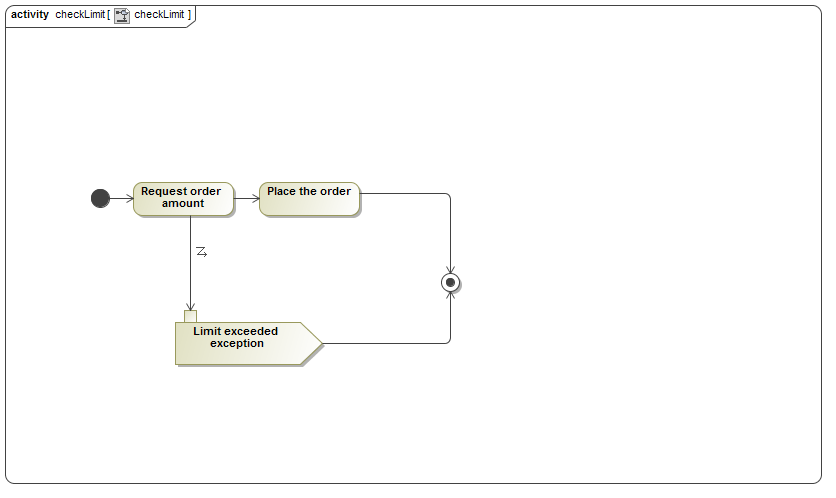
\includegraphics[width=1.0\textwidth]{../images/checkLimit.png}
    \caption{The activity diagram for checking limits} 
\end{figure}

\begin{figure}[H]
	\centering
	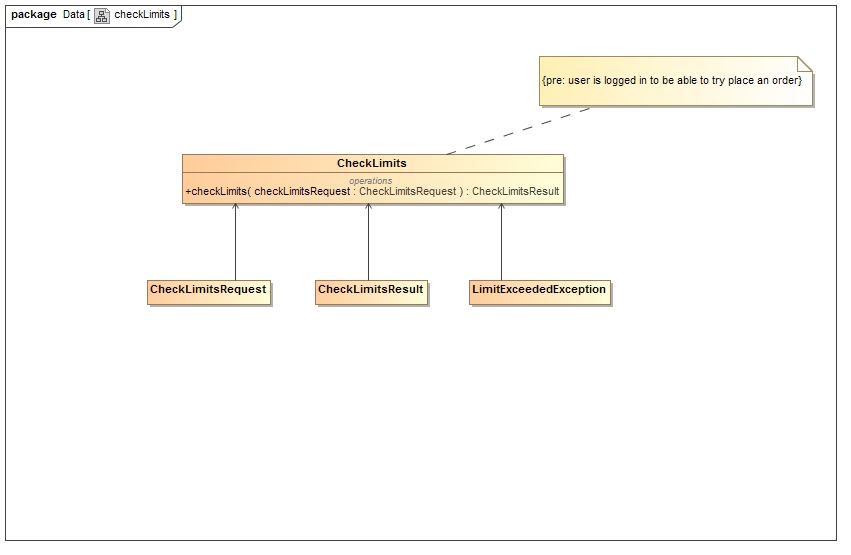
\includegraphics[width=1.0\textwidth]{../images/checkLimitsSC.jpg}
	\caption{The service contract for checking limits}
\end{figure}

\subsection{Manage Inventory Module}
The inventory module is where the cafeteria manager will keep track of stock additions and removals. Different menu items require certain inventory items.This use case diagram indicates the functionality around adding, deleting, searching for and updating inventory.
\begin{figure}[H]
  \centering
    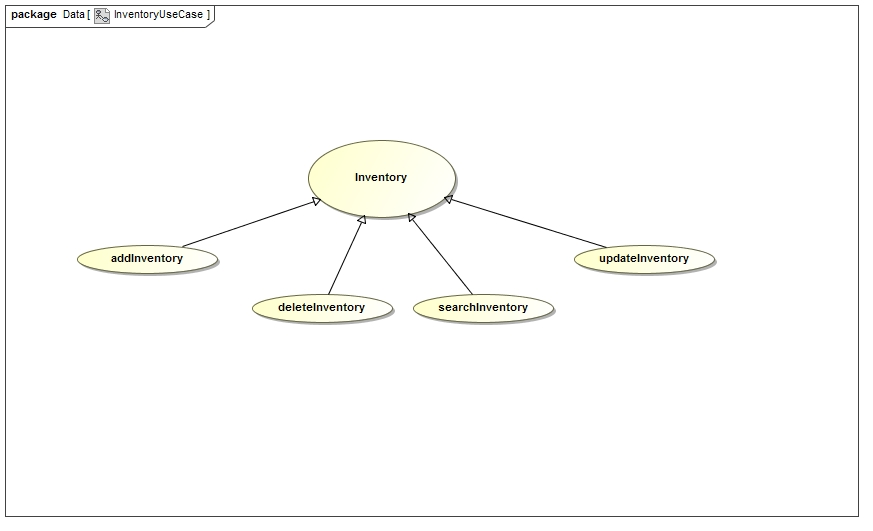
\includegraphics[width=1.0\textwidth]{../images/InventoryUseCase.jpg}
    \caption{The use case for inventory} 
\end{figure}

\subsubsection{addInventory}
The service contract and activity diagram for addInventory to follow. addInventory falls under the use case for Inventory (refer to page   figure   to view this use case diagram). The cafeteria manager will be able to manage inventory items via the allocated page.
\begin{figure}[H]
  \centering
    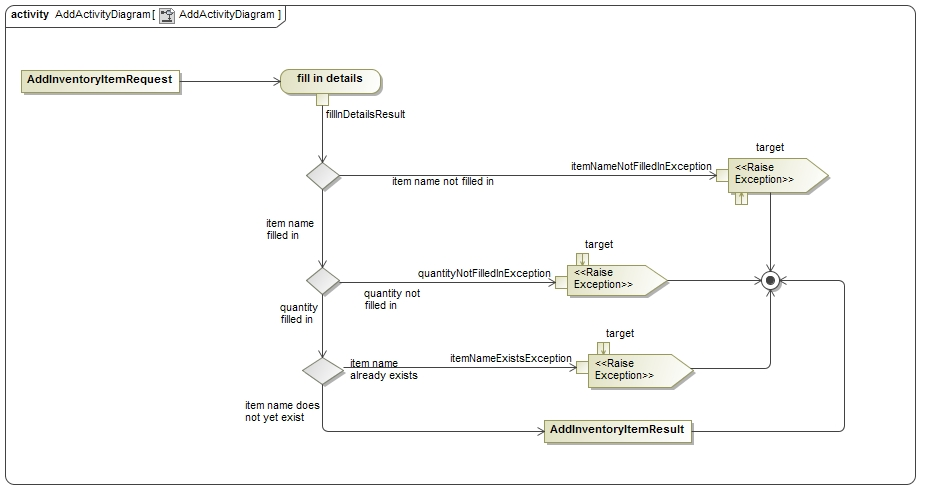
\includegraphics[width=1.0\textwidth]{../images/AddActivityDiagram.jpg}
    \caption{The activity diagram for adding inventory} 
\end{figure}

\begin{figure}[H]
	\centering
	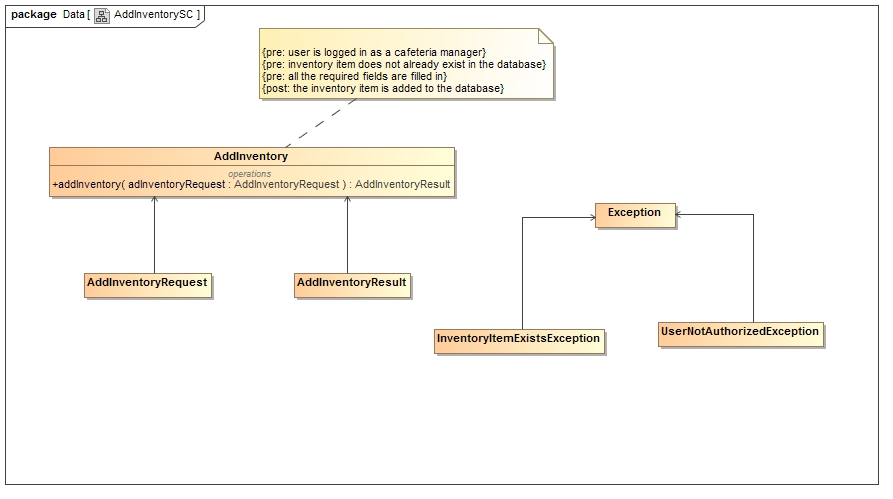
\includegraphics[width=1.0\textwidth]{../images/AddInventorySC.jpg}
	\caption{The service contract for adding inventory}
\end{figure}

\subsubsection{searchInventory}
The service contract and activity diagram for searchInventory to follow. searchInventory falls under the use case for Inventory (refer to page   figure   to view this use case diagram). The cafeteria manager will be able to search for inventory items via the allocated page and from there be able to delete or update them.
\begin{figure}[H]
  \centering
    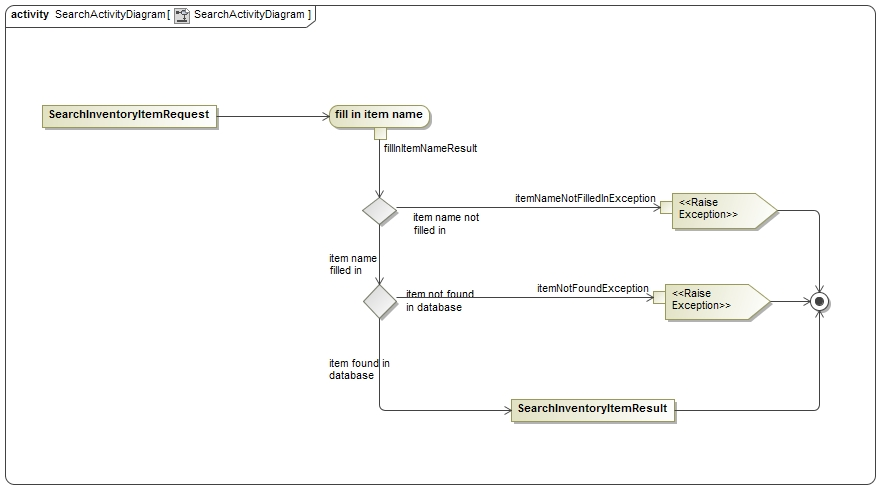
\includegraphics[width=1.0\textwidth]{../images/SearchActivityDiagram.jpg}
    \caption{The activity diagram for searching for inventory} 
\end{figure}

\begin{figure}[H]
	\centering
	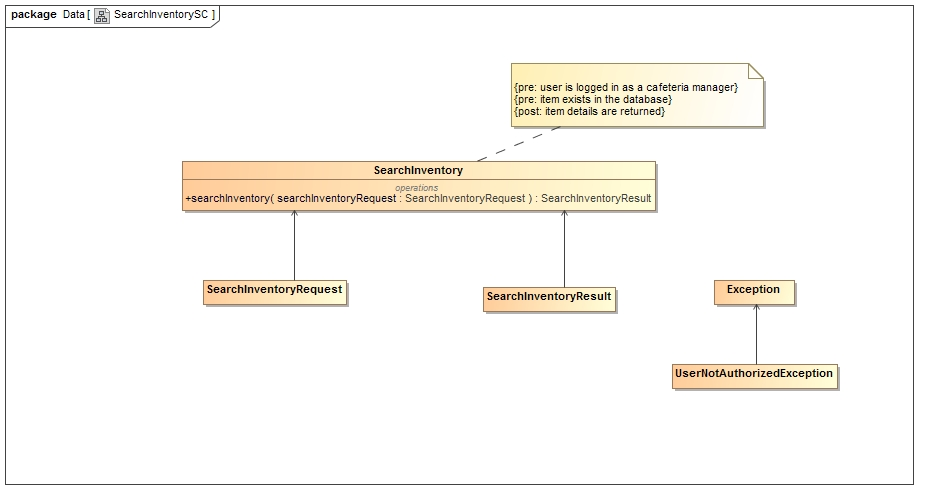
\includegraphics[width=1.0\textwidth]{../images/SearchInventorySC.jpg}
	\caption{The service contract for searching for inventory}
\end{figure}

\subsubsection{deleteInventory}
The service contract and activity diagram for deleteInventory to follow. deleteInventory falls under the use case for Inventory (refer to page   figure   to view this use case diagram). The cafeteria manager will be able to delete inventory items via the allocated page.
\begin{figure}[H]
  \centering
    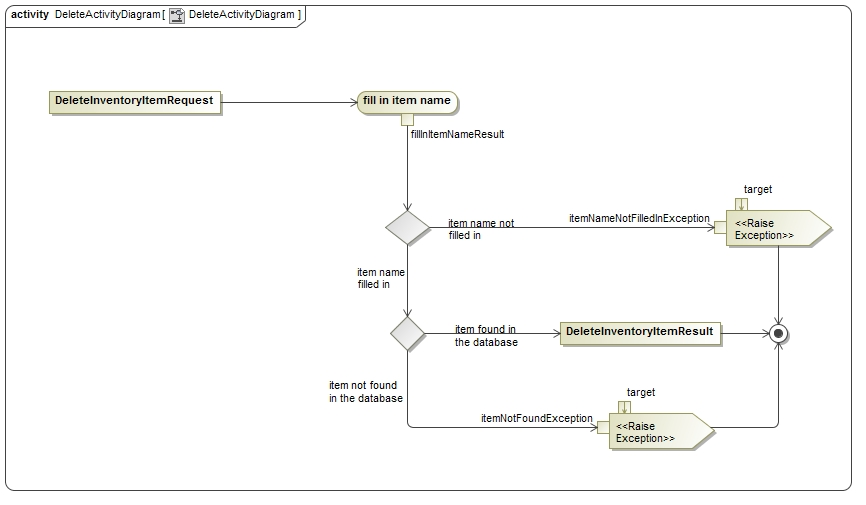
\includegraphics[width=1.0\textwidth]{../images/DeleteActivityDiagram.jpg}
    \caption{The activity diagram for adding inventory} 
\end{figure}

\begin{figure}[H]
	\centering
	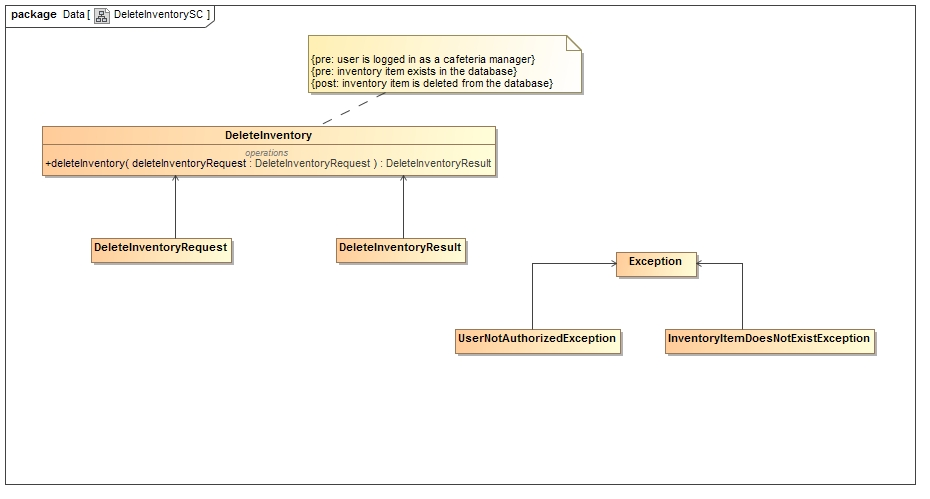
\includegraphics[width=1.0\textwidth]{../images/DeleteInventorySC.jpg}
	\caption{The service contract for adding inventory}
\end{figure}

\subsubsection{updateInventory}
The service contract and activity diagram for updateInventory to follow. updateInventory falls under the use case for Inventory (refer to page   figure   to view this use case diagram). The cafeteria manager will be able to update inventory items via the allocated page.
\begin{figure}[H]
  \centering
    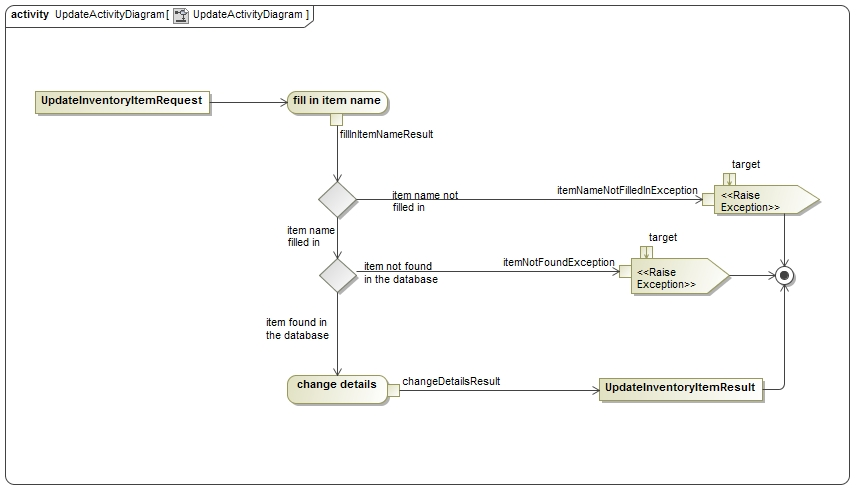
\includegraphics[width=1.0\textwidth]{../images/UpdateActivityDiagram.jpg}
    \caption{The activity diagram for updating inventory} 
\end{figure}

\begin{figure}[H]
	\centering
	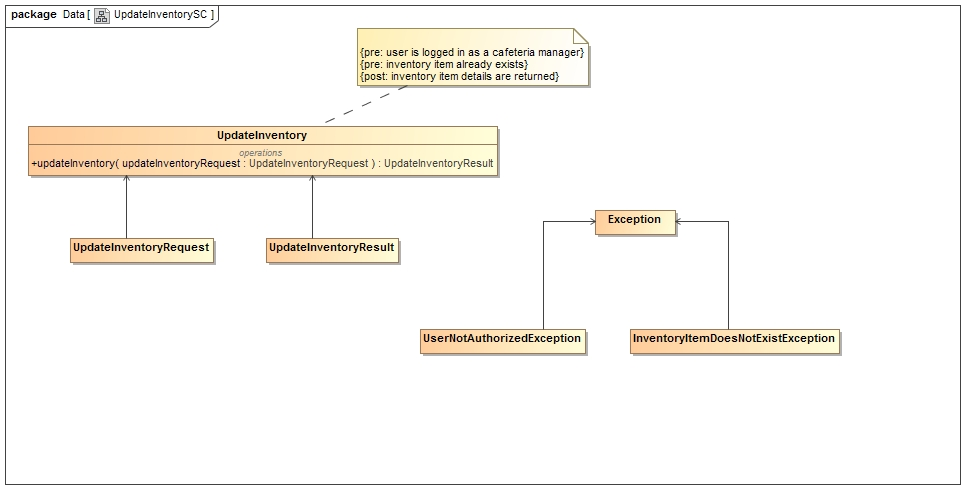
\includegraphics[width=1.0\textwidth]{../images/UpdateInventorySC.jpg}
	\caption{The service contract for updating inventory}
\end{figure}

\subsection{Manage Profile Module}
 The user will be allowed to customize various settings such as resetting his/her personal limit, changing password and email, displaying the bill and viewing favourites. The following use case diagram indicates the above mentioned functionality around managing the profile. Hence, it has the use cases generateFavourite and edit profile.

\begin{figure}[H]
  \centering
    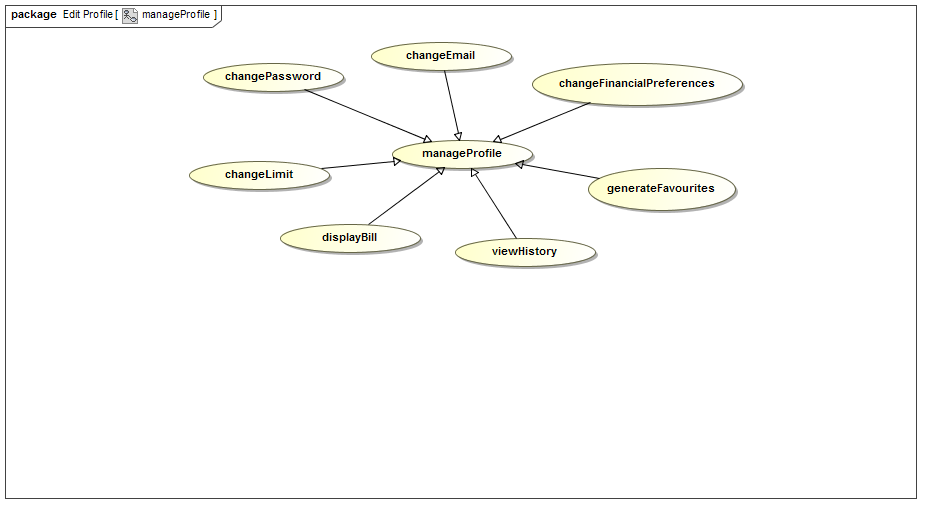
\includegraphics[width=1.0\textwidth]{../Diagrams/ManageProfile/manageProfileUseCase.png}
    \caption{The use case diagram for managing profile} 
\end{figure}

\subsubsection{setFinancialPreferences}
The service contract and activity diagram for setFinancialPreferences to follow. setFinancialPreferences falls under the use case for Manage Profile (refer to page 24 figure 22 to view this use case diagram). The user will be able to choose where their monthly bill  is sent to.
\begin{figure}[H]
  \centering
    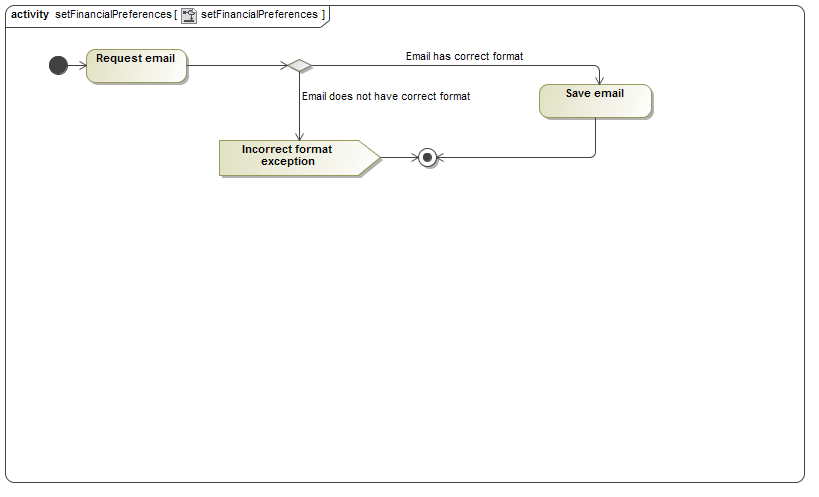
\includegraphics[width=1.0\textwidth]{../Diagrams/ManageProfile/ActivityDiagrams/setFinancialPreferences1.png}
    \caption{The activity diagram for setting financial preferences} 
\end{figure}

\begin{figure}[H]
	\centering
	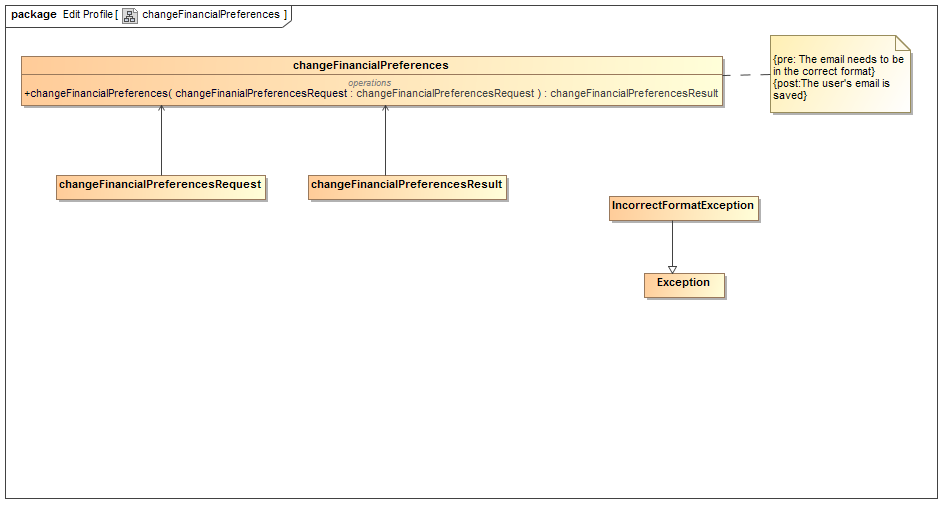
\includegraphics[width=1.0\textwidth]{../Diagrams/ManageProfile/serviceContracts/changeFinancialPreferencesServiceContract.png}
	\caption{The service contract for settting financial preferences}
\end{figure}

\subsubsection{changePassword}
The service contract and activity diagram for changePassword follow. changePassword falls under the use case for Edit Profile (refer to page 24 figure 22 to view this use case diagram). The user will be able to edit their password.
\begin{figure}[H]
  \centering
    \includegraphics[width=1.0\textwidth]{../Diagrams/ManageProfile/ActivityDiagrams/setPassword1.png}
    \caption{The activity diagram for changing password} 
\end{figure}
	
\begin{figure}[H]
	\centering
	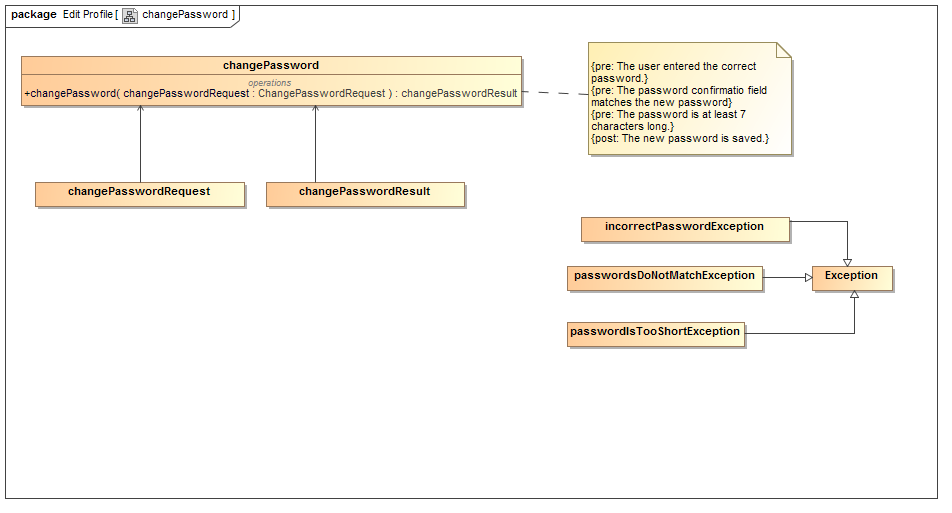
\includegraphics[width=1.0\textwidth]{../Diagrams/ManageProfile/serviceContracts/changePasswordServiceContract.png}
	\caption{The service contract for changing password}
\end{figure}

\subsubsection{changeEmail}
The service contract and activity diagram for changeEmail follow. changeEmail falls under the use case for Edit Profile (refer to page 24 figure 22 to view this use case diagram). The user will be able to edit their email address.
\begin{figure}[H]
  \centering
    \includegraphics[width=1.0\textwidth]{../Diagrams/ManageProfile/ActivityDiagrams/setEmail1.png} 
    \caption{The activity diagram for changing email address}
\end{figure}
	
\begin{figure}[H]
	\centering
	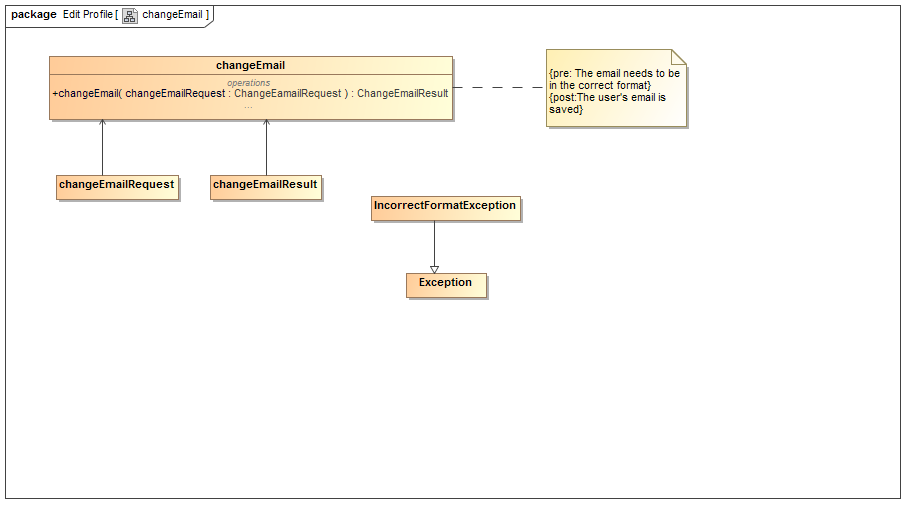
\includegraphics[width=1.0\textwidth]{../Diagrams/ManageProfile/serviceContracts/changeEmailServiceContract.png}
	\caption{The service contract for changing email address}
\end{figure}

\subsubsection{changeLimit}
The service contract and activity diagram for changeLimit follow. changeLimit falls under the use case for Edit Profile (refer to page 24 figure 22 to view this use case diagram). The user will be able to change their personal spending limit on their profile, however, this must not exeed the system's limit.
\begin{figure}[H]
  \centering
    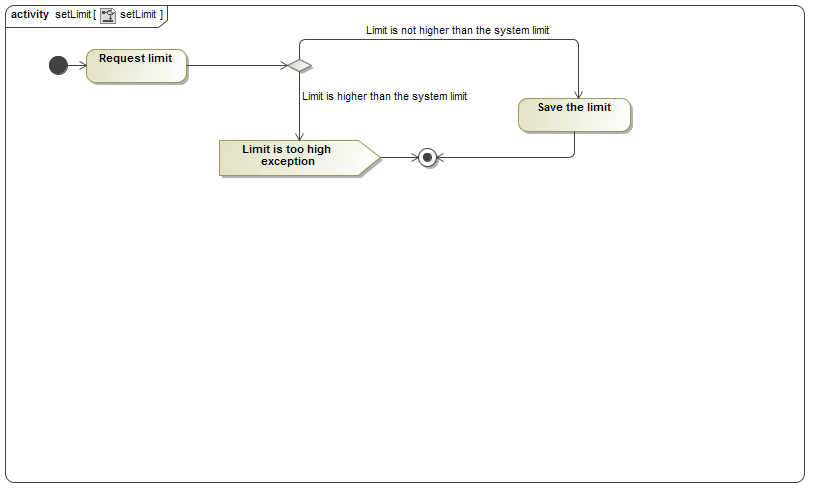
\includegraphics[width=1.0\textwidth]{../Diagrams/ManageProfile/ActivityDiagrams/setLimit.png}
    \caption{The activity diagram for setting limit} 
\end{figure}

\begin{figure}[H]
	\centering
	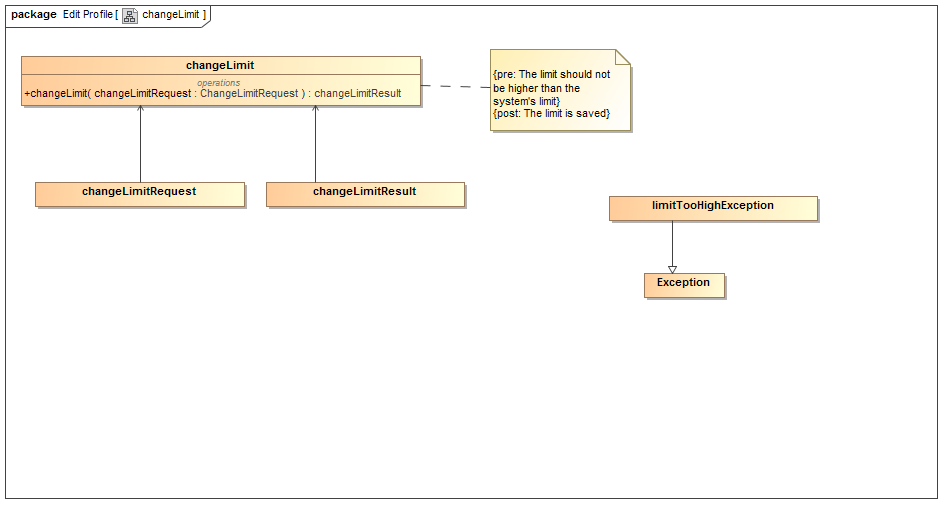
\includegraphics[width=1.0\textwidth]{../Diagrams/ManageProfile/serviceContracts/changeLimitServiceContract.png}
	\caption{The service contract for setting limit}
\end{figure}
 
\subsection{Manage System Module}
 The superuser will be allowed to customize various settings such as assign roles to the users, changing employee IDs, setting the maximum spending limit as well as branding settings such as setting the canteen name and changing the cover photo. The following use case diagram indicates the above mentioned functionality.

\begin{figure}[H]
  \centering
    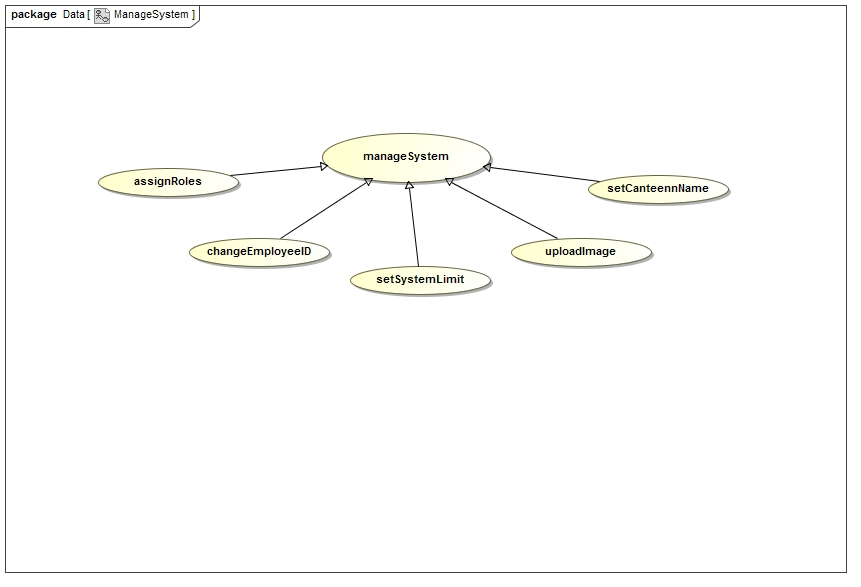
\includegraphics[width=1.0\textwidth]{../images/ManageSystem.jpg}
    \caption{The use case diagram for managing system} 
\end{figure}

\subsubsection{assignRoles}
The service contract and activity diagram for assignRoles to follow. assignRoles falls under the use case for Manage System (refer to page   figure   to view this use case diagram). The superuser is the only user who can allocate the various roles to users. Roles consist of finance managers, cashiers, cafeteria managers, and administrator. 
\begin{figure}[H]
  \centering
    \includegraphics[width=1.0\textwidth]{../Diagrams/ManageProfile/ActivityDiagrams/setFinancialPreferences1.png}
    \caption{The activity diagram for assign roles} 
\end{figure}

\begin{figure}[H]
	\centering
	\includegraphics[width=1.0\textwidth]{../Diagrams/ManageProfile/serviceContracts/changeFinancialPreferencesServiceContract.png}
	\caption{The service contract for assign roles}
\end{figure}

\subsubsection{changeEmployeeID}
The service contract and activity diagram for changeEmployeeID to follow. changeEmployeeID falls under the use case for Manage System (refer to page   figure   to view this use case diagram). The superuser is the only user who can change the employee ID of employees if they typed their ID incorrectly or if the company changes the IDs.
\begin{figure}[H]
  \centering
    \includegraphics[width=1.0\textwidth]{../images/changeEmployeeIDActivityDiagram.png}
    \caption{The activity diagram for change employee ID} 
\end{figure}

\begin{figure}[H]
	\centering
	\includegraphics[width=1.0\textwidth]{../images/changeEmployeeIdSC.png}
	\caption{The service contract for change employee ID}
\end{figure}

\subsubsection{setSystemWideLimit}
The service contract and activity diagram for setSystemWideLimit to follow. setSystemWideLimit falls under the use case for Manage System (refer to page   figure   to view this use case diagram). The superuser is the only user who can change the maximum monthly spending limit. Users will then not be able to set their personal monthly spending limits to a value higher than this.
\begin{figure}[H]
  \centering
    \includegraphics[width=1.0\textwidth]{../images/changeEmployeeIDActivityDiagram.png}
    \caption{The activity diagram for setting the system wide limit} 
\end{figure}

\begin{figure}[H]
	\centering
	\includegraphics[width=1.0\textwidth]{../images/setSystemWideLimit.png}
	\caption{The service contract for setting the system wide limit}
\end{figure}

\subsubsection{setCanteenName}
The service contract and activity diagram for setCanteenName to follow. setCanteenName falls under the use case for Manage System (refer to page   figure   to view this use case diagram). The superuser can change the canteen name hence not restricting the system to be used at only one canteen - making the system portable. 
\begin{figure}[H]
  \centering
    \includegraphics[width=1.0\textwidth]{../images/SetCanteenNameActivity.png}
    \caption{The activity diagram for setting the canteen name} 
\end{figure}

\begin{figure}[H]
	\centering
	\includegraphics[width=1.0\textwidth]{../images/SetCanteenServiceContract.png}
	\caption{The service contract for setting the canteen name}
\end{figure}

\subsubsection{uploadImage}
The service contract and activity diagram for uploadImage to follow. uploadImage falls under the use case for Manage System (refer to page   figure   to view this use case diagram). The superuser can change the canteen cover photo hence not restricting the system to be used at only one canteen - making the system portable. 
\begin{figure}[H]
  \centering
    \includegraphics[width=1.0\textwidth]{../images/UploadImageActivityDiagram.jpg}
    \caption{The activity diagram for uploading a cover image} 
\end{figure}

\begin{figure}[H]
	\centering
	\includegraphics[width=1.0\textwidth]{../images/UploadImageSC.jpg}
	\caption{The service contract for uploading a cover image}
\end{figure}


\section{Comment}
No comment for this version update.

\end{document}

